\newcommand{\cm}{\mathrm{cm^{-1}}}
\newcommand{\nm}{\mathrm{nm}}
\newcommand{\pltw}{0.8\textwidth}
\section{Evaluation}

\subsection{Measuring bias of spectrometer}
To be able to identify the absorbtion spectrum of the iodine 2 molecule, we have to analise 
the measurements for callibration with the Na- and Hg-vapour lamps, respectively. The measured
spectrum over the entire range of the spectrometer is plotted in figure \ref{fig:specturm_all}. 
To locate the maxima, we magnify the recordings in a region around the corrispoding maximum. 
For sodium, this is done in figure \ref{fig:na_max}. One can see the two characteristic peaks 
at 
\begin{eqnarray*}
    \lambda_\mathrm{max, 1} = 589.1 \pm 0.6 \nm \\
    \lambda_\mathrm{max, 2} = 589.6 \pm 0.6 \nm.
\end{eqnarray*}
The uncertainty of 0.6nm ist taken from the value given in \cite{}, being higher than the 
one stemming from limited sharpness of the maxima (fwhm about 0.4nm as seen in the figures). 
These corrispond with the values given in literature \cite{}, namely 
\begin{eqnarray*}
    \lambda_\mathrm{max, 1} = 589.0 \nm \\
    \lambda_\mathrm{max, 2} = 589.6 \nm.
\end{eqnarray*}
In the recorded spectrum, we also se another, smaller peak at 
\begin{equation}
    \lambda = 588.4 \pm 0.6 \nm.
\end{equation} 
This peak is not found in literature and seems to be an artefact of the measurement. 
In fact, as the light from the Na lamp was not colliminated and focused very well, one could 
suspect diffration at the entrance of the spectrometer as the cause, as the spectrometer 
doesn't measure wavelength directly but rather the intensity corrisponding to a certain angle. 

For the Hg lamp, we observe similar results. As seen in \ref{fig:spectrum_all}, intensities 
of the minima varied quiet drastically. For that reason, we took various measurements of which 
we can use one for the first maximum (fig. \ref{fig:hg1_max}) and another at much lower 
intensity for the three other ones (fig. \ref{fig:hg1_max}). We identify the following maxima:
\begin{eqnarray*}
    \lambda_\mathrm{max, 1} &=& 435.5 \pm 0.6 \ (435.83)\nm \\
    \lambda_\mathrm{max, 2} &=& 545.9 \pm 0.6 \ (545.9)\nm \\
    \lambda_\mathrm{max, 3} &=& 576.8 \pm 0.6 \ (576.8)\nm \\
    \lambda_\mathrm{max, 4} &=& 576.9 \pm 0.6 \ (576.9)\nm.
\end{eqnarray*}
The values in parenthesis cite literature values \cite{}. \\
As the spectrometer yields results lying within the literature values for the states error 
of 0.6nm, we conclude that there is no bias in the measured wavelength. 

\begin{figure}
\centering
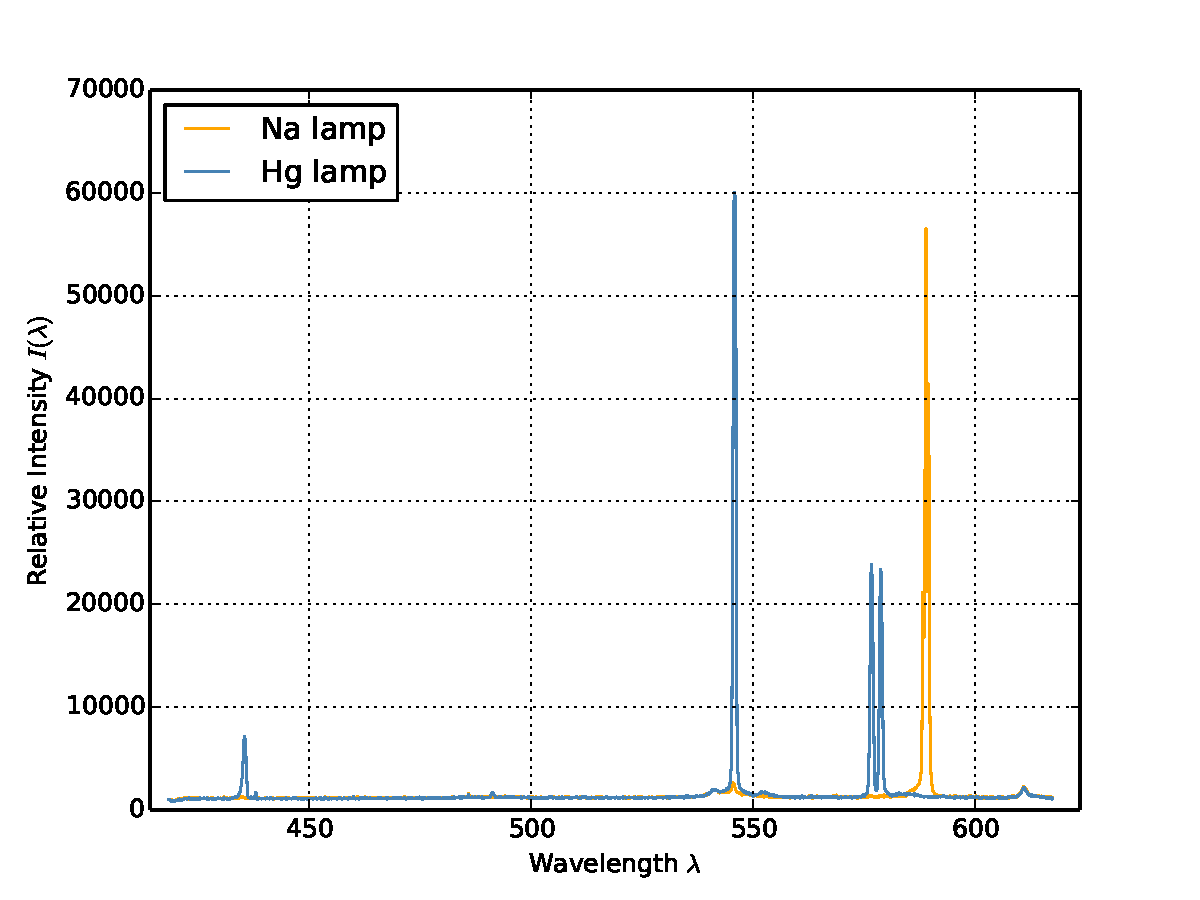
\includegraphics[width=\pltw]{analysis/figures/spectrum_all.pdf}
\caption{Measured spectrum of Na and Hg lamp}
\label{fig:spectrum_all}
\end{figure}

\begin{figure}
\centering
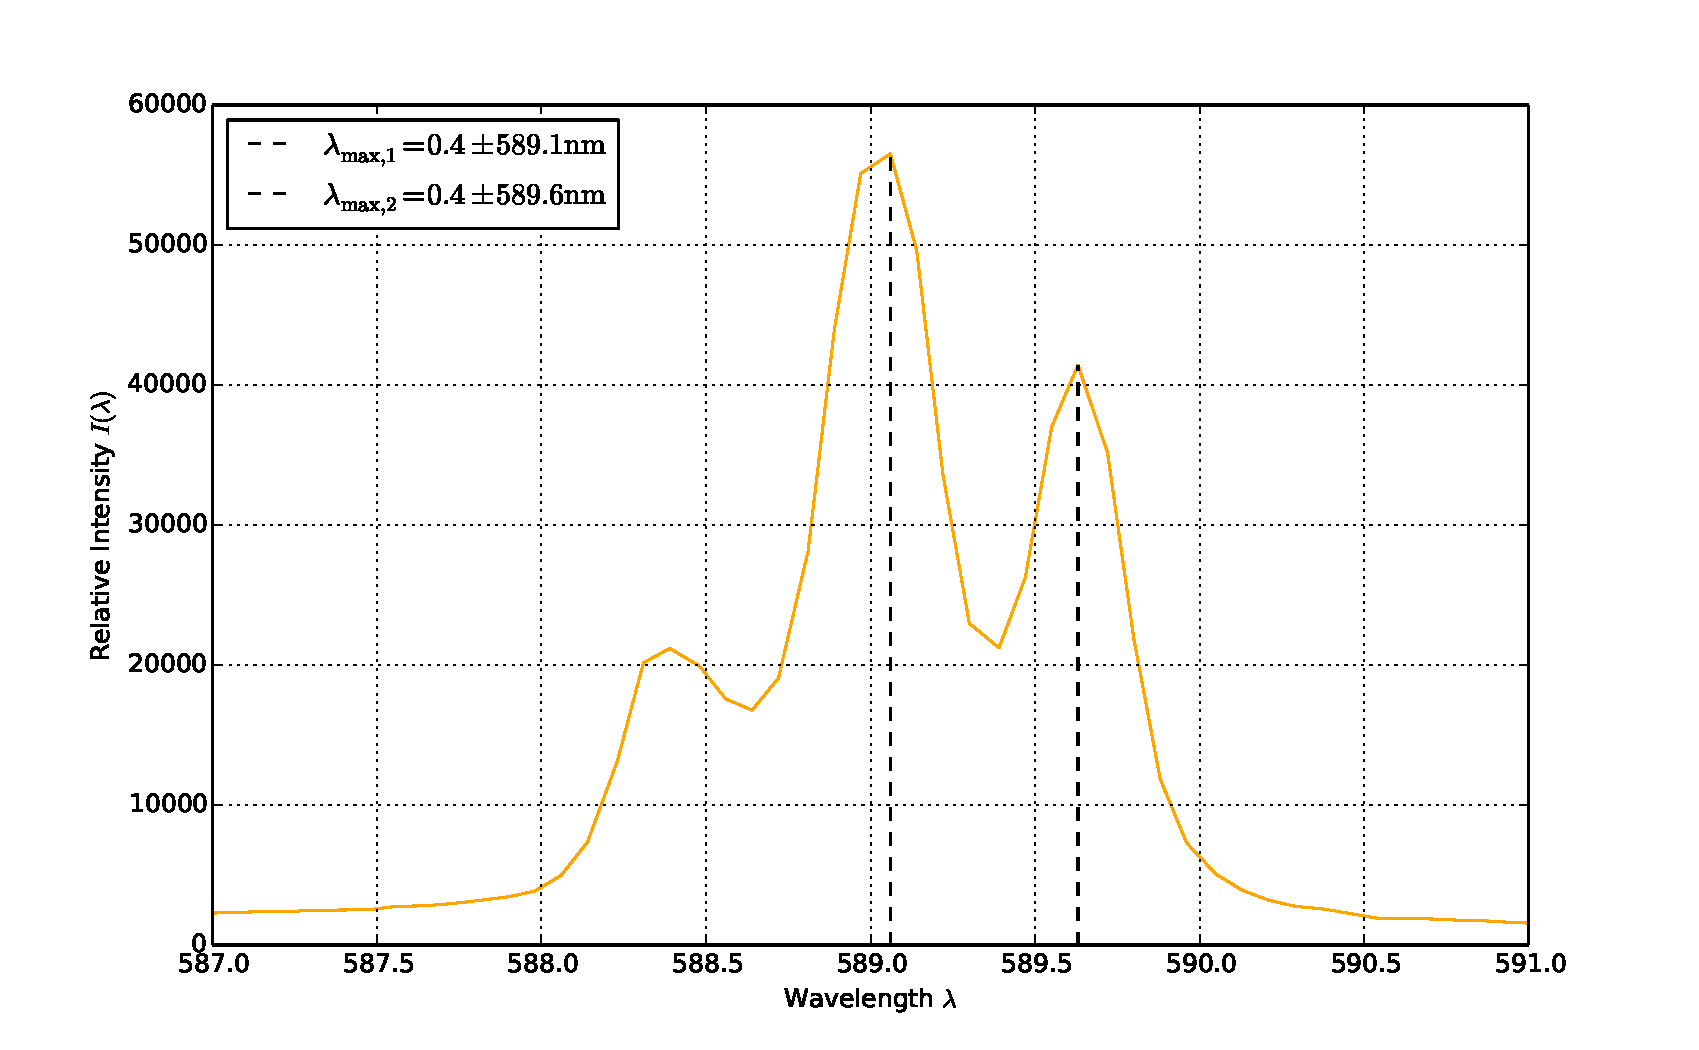
\includegraphics[width=\pltw]{analysis/figures/na_max.pdf}
\caption{Measured spectrum of the Na lamp, detail at the 
characteristic orange double line}
\label{fig:na_max}
\end{figure}

\begin{figure}
\centering
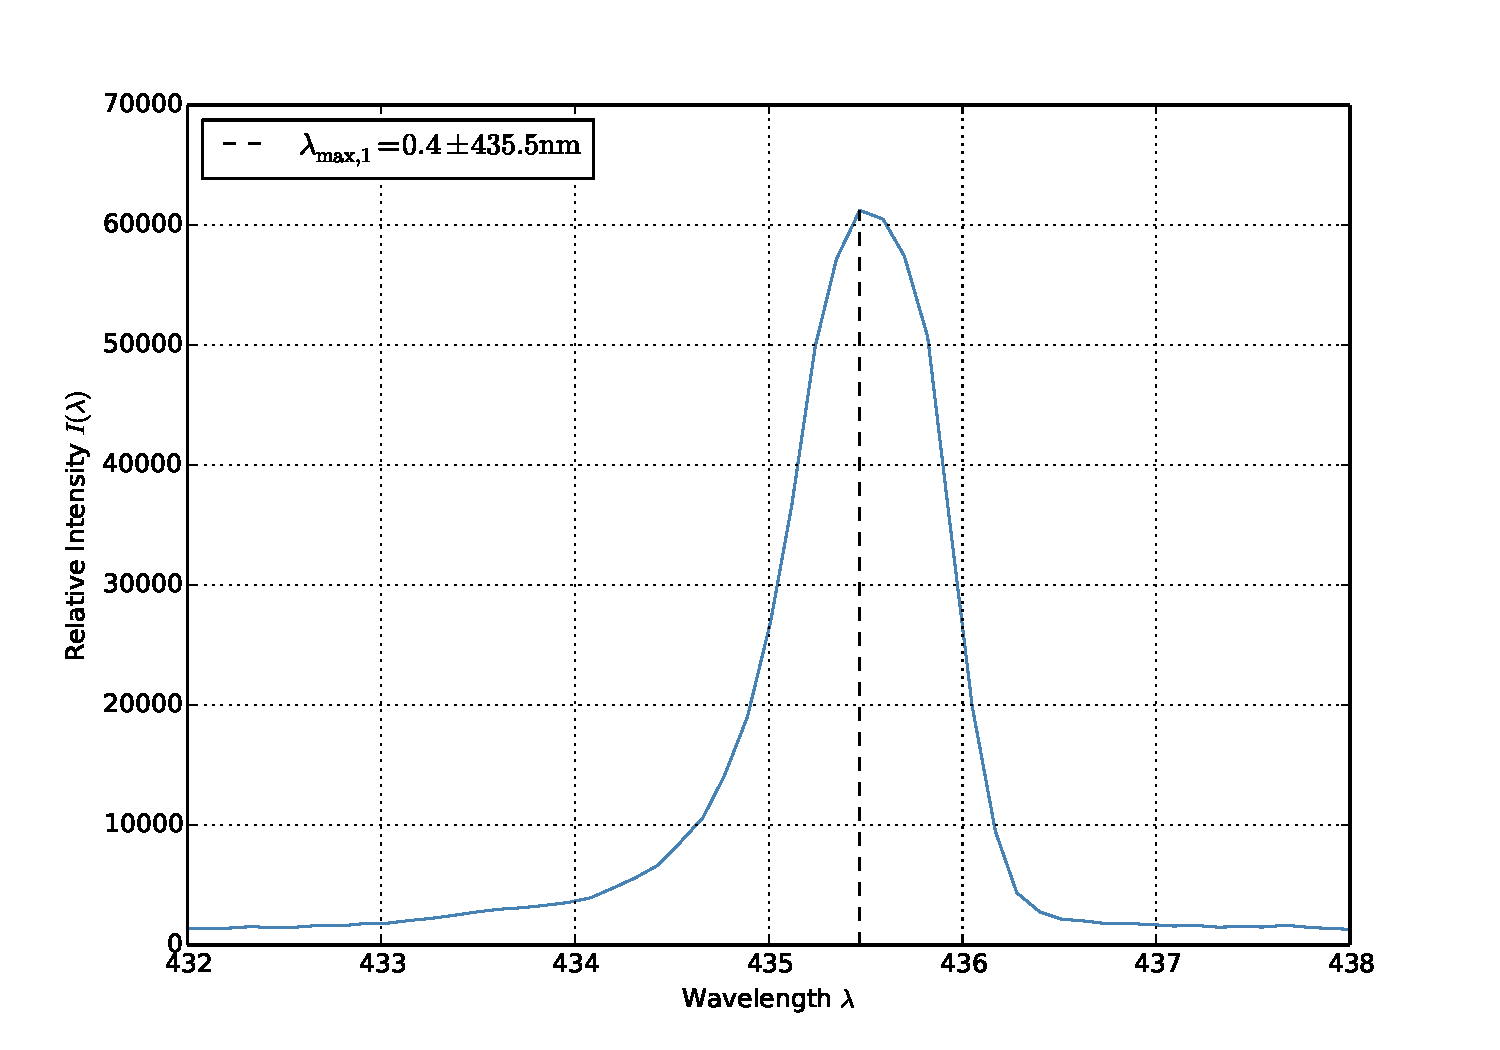
\includegraphics[width=\pltw]{analysis/figures/hg1_max.pdf}
\caption{Measured spectrum of the hg lamp, detail at first maximum}
\label{fig:hg1_max}
\end{figure}

\begin{figure}
\centering
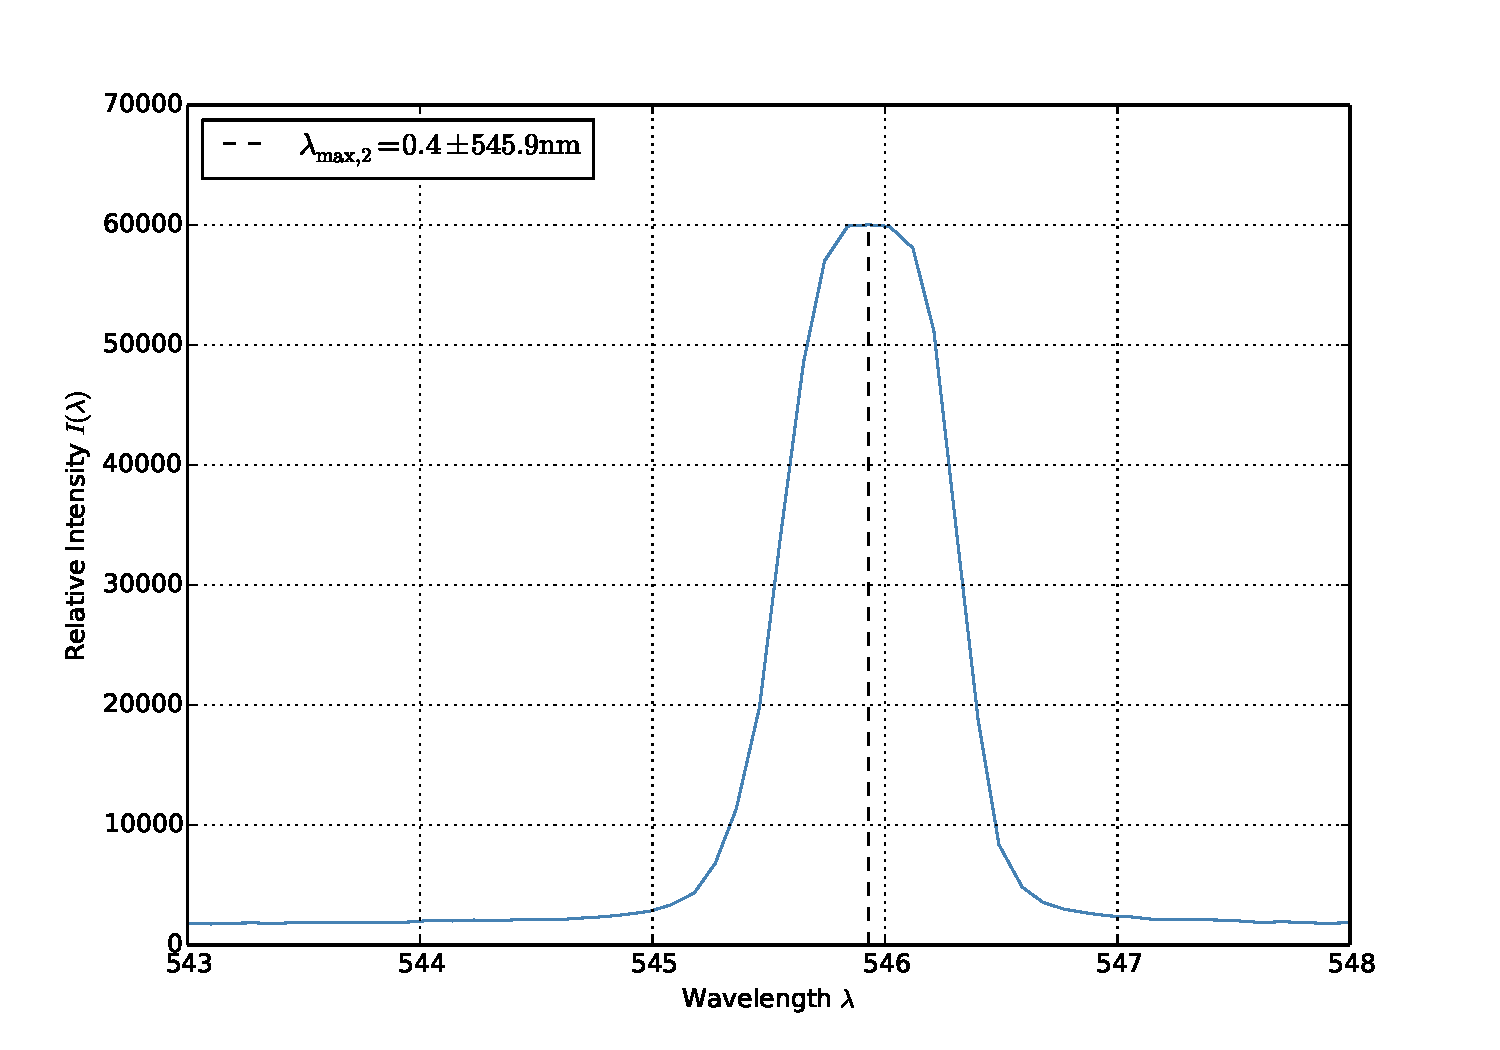
\includegraphics[width=\pltw]{analysis/figures/hg2_max.pdf}
\caption{Measured spectrum of the hg lamp, detail at second maximum}
\label{fig:hg2_max}
\end{figure}

\begin{figure}
\centering
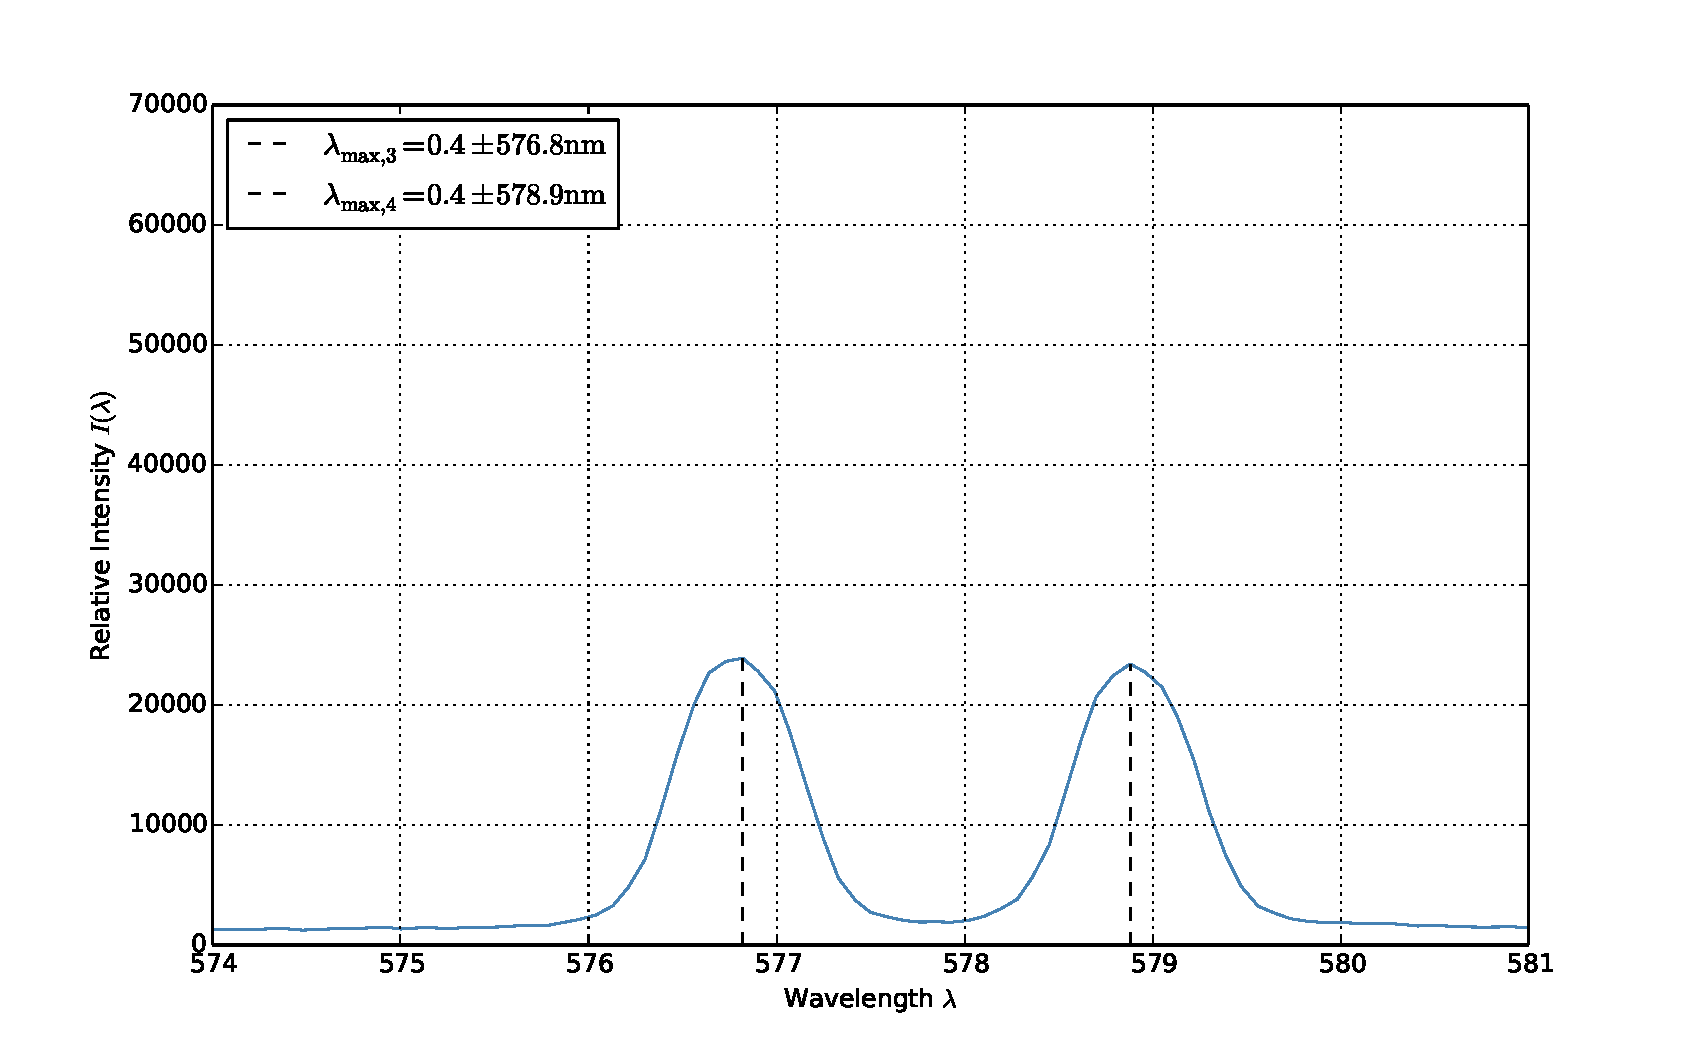
\includegraphics[width=\pltw]{analysis/figures/hg3_max.pdf}
\caption{Measured spectrum of the hg lamp, detail at thrid and fourth maximum}
\label{fig:hg3_max}
\end{figure}

\subsection{Spectrum of halogen lamp}
As we look out to measure the absorbtion spectrum of iodine, we first take a quick look at 
the specturm of the background from which photons are to be absorbed. The measured spectrum 
of the used halogen lamp within the range of wavelength in question is shown in figure 
\ref{fig:specturm_halogen_full}.
\begin{figure}
\centering
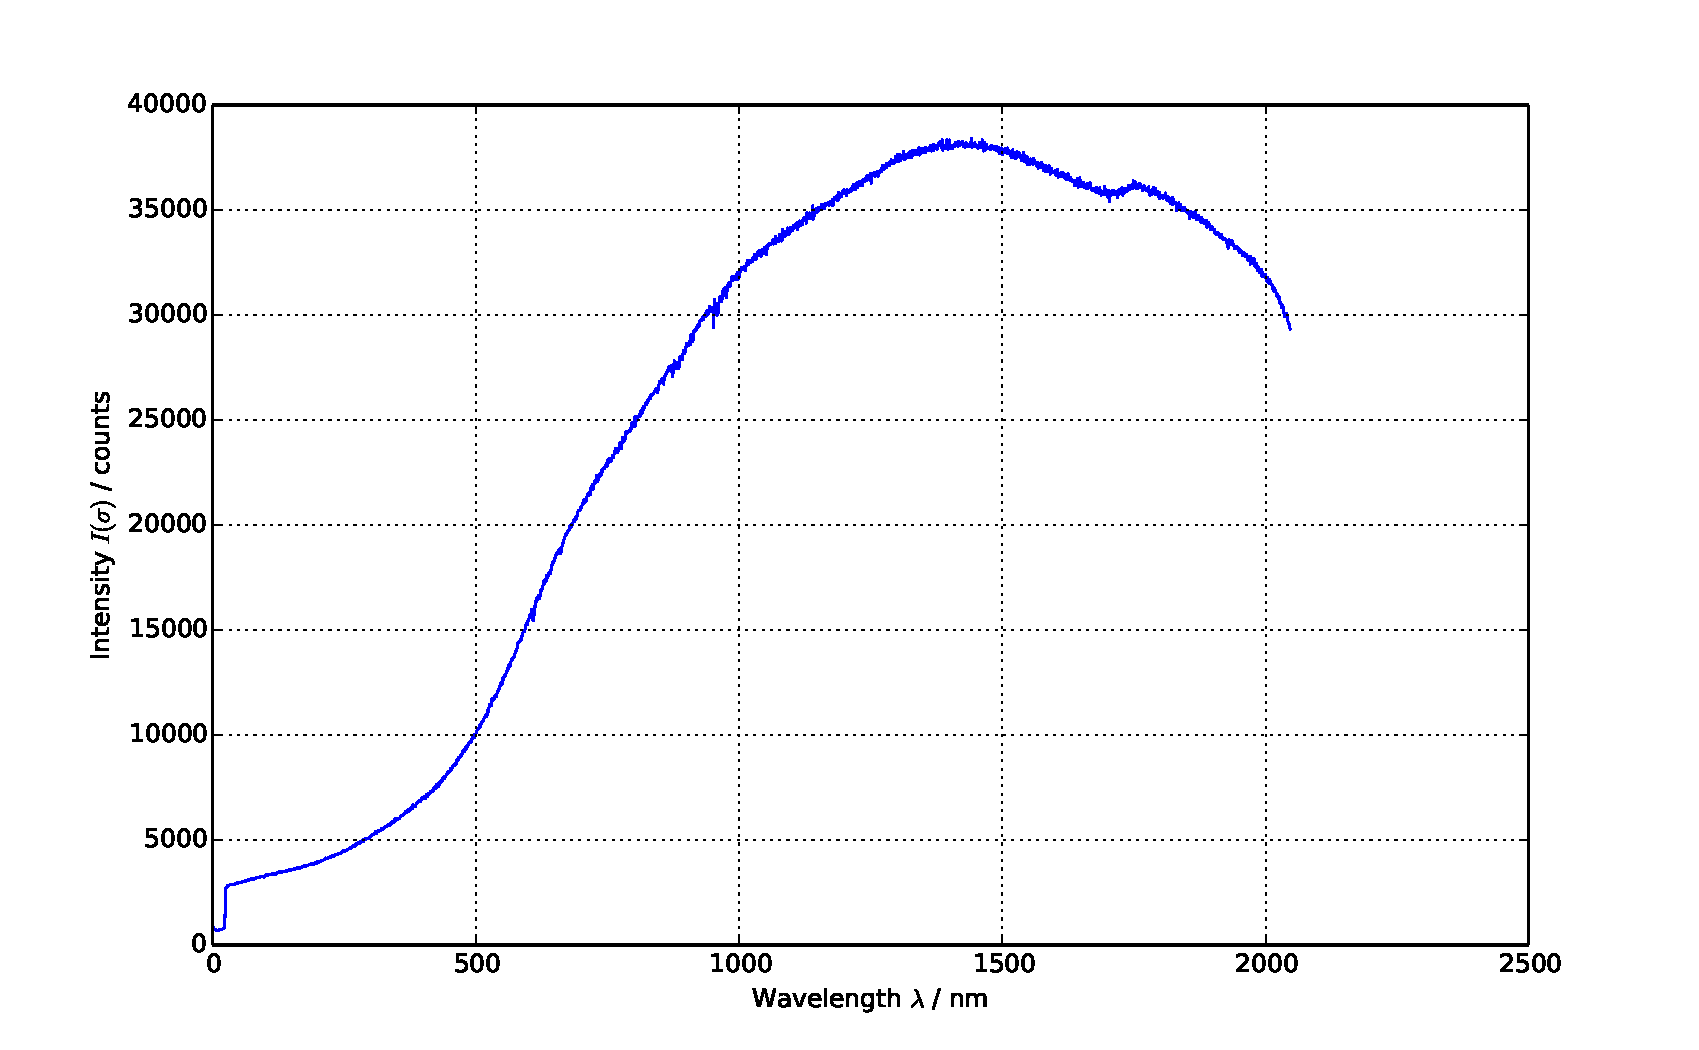
\includegraphics[width=\pltw]{analysis/figures/halogen_02.pdf}
\caption{Measured spectrum of the halogen lamp over the entire spectrum, no coerrection for 
diffraction in light}
\label{fig:spectrum_halogen_full}
\end{figure}
To be able to compare this to the absorbtion spectrum, we firth need to make the same 
corrections for diffraction in light as we do for the latter. We do so by linearly 
interpolating given literature values of the diffaction indice, given in table 
\ref{tab:diff_air}.

\begin{table}[h]
\centering
\begin{tabular}{| c |l|l|l|l|}
\hline
$\lambda [\nm]$              & 680  & 600  & 540  & 500 \\ \hline
$(n_\mathrm{air} - 1) \cdot 10^{-4}$ & 2.76 & 2.77 & 2.78 & 279 \\ \hline
\end{tabular}
\caption{Diffraction indices for air at room temperatur and normal pressure for chosen wavelength $\lambda$, taken from \cite{}.}
\label{tab:diff_air}
\end{table}
The linear interpolation is done by the following equation:

\begin{eqnarray*}
    n_\lambda &=& \frac{(2.79 - 0.01  j)}{10 ^{4}} - \
    \frac{(\lambda - \lambda_\mathrm{lower})} {10^{6} \cdot \
(\lambda_\mathrm{upper} - \lambda_\mathrm{lower})} + 1 \\
    \lambda &=& n_\lambda \, \lambda
\end{eqnarray*}
where j is the index of the collum of table \ref{tab:diff_air} within which $\lambda$ lies, 
$\lambda_\mathrm{upper}$ and $\lambda_\mathrm{lower}$ are the upper and lower bounds of the 
intervall (more precisely: $\lambda \in (\lambda_\mathrm{upper}, \lambda_\mathrm{lower}]$ ). 

The corrected values of $\lambda$ are now restricted to values of 
$\lambda \in [500\nm, 620\nm]$ and converted to $\cm$ by taking th inverse. The result 
can be observed in figure \ref{"fig:spectrum_halogen_red"}.
\begin{figure}
\centering
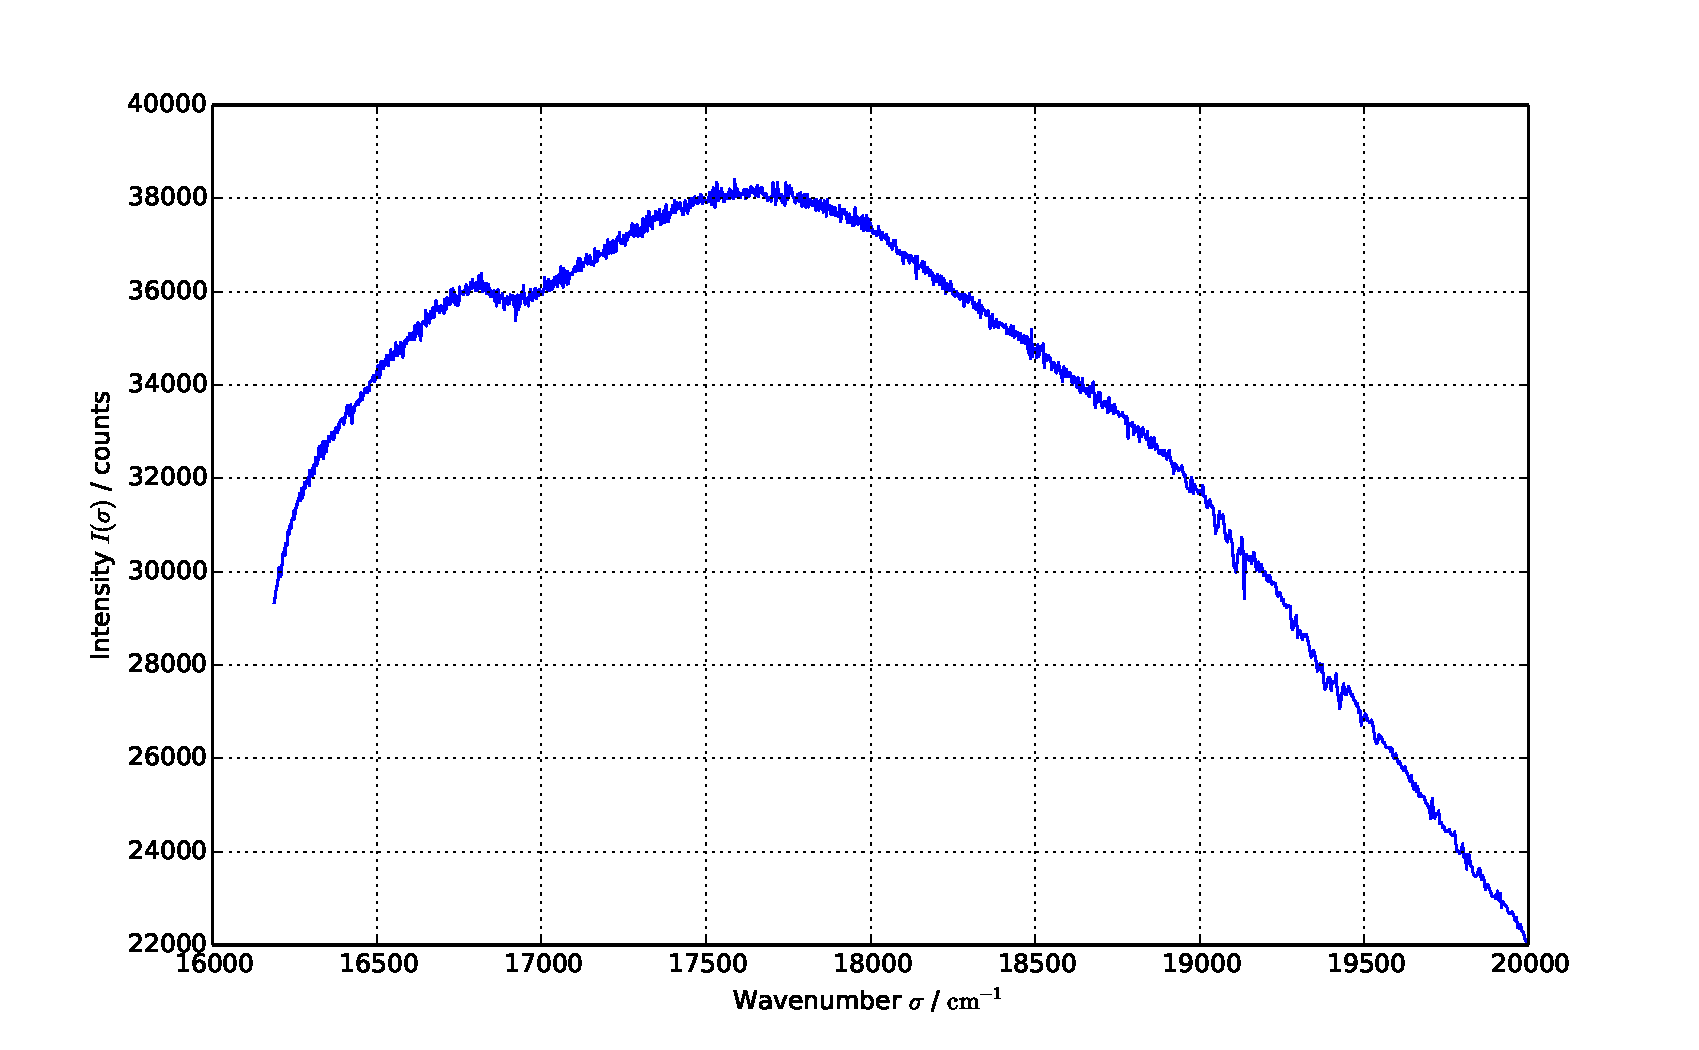
\includegraphics[width=\pltw]{analysis/figures/halogen_red.pdf}
\caption{Measured spectrum of the halogen lamp over the entire spectrum, no correction for 
diffraction in light}
\label{fig:spectrum_halogen_red}
\end{figure}
